\documentclass[11pt]{article}

% cs250preamble.tex --- shared preamble for CS 250 course notes
%
% This file is \input by main.tex and by each individual module
% file so that each module can still compile standalone. Any
% package or custom-environment change should be made here, not
% in the individual module files.

\usepackage[T1]{fontenc}
\usepackage[margin=1in]{geometry}
\usepackage{amsmath, amssymb, amsthm}
\usepackage{enumitem}
\usepackage{hyperref}
\usepackage{booktabs}
\usepackage{listings}
\usepackage{xcolor}
\usepackage{tikz}
\usetikzlibrary{shapes.geometric, shapes.gates.logic.US, shapes.gates.logic.IEC, arrows.meta, positioning, calc, trees}
\usepackage{bussproofs}
\usepackage{mdframed}

\lstset{
  basicstyle=\ttfamily\small,
  frame=single,
  breaklines=true,
  columns=fullflexible,
  mathescape=true
}

\theoremstyle{definition}
\newtheorem{theorem}{Theorem}[section]
\newtheorem{definition}[theorem]{Definition}
\newtheorem{example}[theorem]{Example}

\hypersetup{
  colorlinks=true,
  linkcolor=blue!60!black,
  urlcolor=blue!60!black
}

% Key-takeaway box: used at the end of major sections and at the end of
% each module to summarise the main points. Expects \item bullets inside.
\newmdenv[
  linewidth=0.8pt,
  linecolor=blue!40!black,
  backgroundcolor=blue!3,
  skipabove=8pt,
  skipbelow=8pt,
  innertopmargin=7pt,
  innerbottommargin=7pt,
  innerleftmargin=9pt,
  innerrightmargin=9pt
]{keytakeawaybox}
\newenvironment{keytakeaway}{%
  \begin{keytakeawaybox}%
  \noindent\textbf{Key takeaways.}%
  \begin{itemize}[leftmargin=1.3em, topsep=2pt, itemsep=1pt, label=\textbullet]%
}{%
  \end{itemize}%
  \end{keytakeawaybox}%
}

% Summary/looking-ahead environment: used once at the end of each module
% to wrap up what the module built and point forward.
\newmdenv[
  linewidth=0.8pt,
  linecolor=gray!60,
  backgroundcolor=gray!5,
  skipabove=8pt,
  skipbelow=8pt,
  innertopmargin=7pt,
  innerbottommargin=7pt,
  innerleftmargin=9pt,
  innerrightmargin=9pt
]{summarybox}

% Sidebar environment: used for tangential asides---historical notes,
% pointers to other areas of math/CS, cross-paradigm remarks---that
% enrich the main narrative without being essential to it. Takes one
% argument: the sidebar's title.
\newmdenv[
  linewidth=0.6pt,
  linecolor=gray!60,
  backgroundcolor=gray!4,
  skipabove=8pt,
  skipbelow=8pt,
  innertopmargin=6pt,
  innerbottommargin=6pt,
  innerleftmargin=9pt,
  innerrightmargin=9pt
]{sidebarbox}
\newenvironment{sidebar}[1]{%
  \begin{sidebarbox}%
  \noindent\textbf{Sidebar: #1.}\par\medskip%
}{%
  \end{sidebarbox}%
}

% Reading-map environment: used at the top of each numbered module to
% indicate Epp coverage, prerequisites, relevant intermezzi, and
% suggested practice problems. Expects four \rmentry{label}{body}
% items inside (or arbitrary paragraphs).
\newmdenv[
  linewidth=0.8pt,
  linecolor=black!55,
  backgroundcolor=yellow!4,
  skipabove=10pt,
  skipbelow=14pt,
  innertopmargin=9pt,
  innerbottommargin=9pt,
  innerleftmargin=11pt,
  innerrightmargin=11pt
]{readingmapbox}
\newcommand{\rmentry}[2]{\par\noindent\textbf{#1}\hspace{0.4em}#2\par}
\newenvironment{readingmap}{%
  \begin{readingmapbox}%
  \noindent{\bfseries\large Reading map}%
  \vspace{2pt}%
  \setlength{\parskip}{4pt plus 1pt}%
}{%
  \end{readingmapbox}%
}


\title{CS 250 --- Preface and Reading Guide}
\author{}
\date{}

\begin{document}
\maketitle

\section*{What this book is}

These notes are a companion to Epp's \emph{Discrete Mathematics with Applications}, fifth edition, for the first term of CS~250. They cover roughly Chapters 1--5 of Epp, reorganized and rewritten from my own idiosyncratic perspective as someone with strong opinions about both logic \emph{and} computer science. They also include several \emph{intermezzi} on topics Epp doesn't cover (Curry--Howard, the algebra of types, the lambda calculus, Gentzen-style natural deduction, quantifiers as games, cardinality, temporal and modal logic) that point toward where the material goes next.

Where Epp and I disagree, it's a somewhat purposeful disagreement based on opinion rather than correctness. This is a very good text, even if I think she's too kind to people who think the natural numbers start with $1$ (pgs. 7--8 of the 5th edition of her book)---a position that is not a difference of opinion but is, as far as I can tell, simply wrong.
\section*{How to use this book}

The book is divided into two kinds of chapters:

\begin{itemize}
  \item \textbf{Numbered modules} (Module 1 through Module 10) form the main spine. They are sequential, in the sense that each module assumes you've understood the previous ones. Every module has a \emph{Reading Map} box at the top telling you which Epp sections it corresponds to, which previous modules are prerequisites, and which intermezzi are relevant.
  \item \textbf{Intermezzi} are unnumbered side trips between modules. They go deeper into topics that are mathematically richer or more computer-sciencey than the main spine requires. They are \textbf{optional} in the sense that exams won't cover them unless your instructor says so---think of them as bonus tracks. The book won't break if you skip them, but most readers find that skipping them makes the main spine feel more arbitrary than it needs to.
\end{itemize}

Each module ends with an \textbf{Exercises section} organized into four tiers:
\begin{itemize}
  \item \textbf{Warm-up}: short, mechanical checks on the definitions. Do them all; they're quick and they catch misreadings.
  \item \textbf{Standard}: typical assignment-style problems. These are where most of the learning happens.
  \item \textbf{Challenge}: problems that ask you to synthesize across the module, or to think a bit harder. Worth discussing with a study partner.
  \item \textbf{Connection}: problems that tie the module to programming, to an intermezzo, or to a later module. Most of these have a Python snippet or a forward-pointer component.
\end{itemize}

Full prose solutions to every exercise are in the \emph{Solutions} appendix. Resist the temptation to look until you've genuinely tried the problem. Reading the solution before attempting the problem is the most common way to feel like you ``get it'' while actually learning nothing.

Each module also has a \textbf{Common mistakes} subsection listing the errors students actually make on that material. Skim it before the assignment; skim it again after you get your grade back.

\section*{Module dependency diagram}

Here's how the modules and intermezzi fit together. Solid arrows are hard prerequisites; dashed arrows are relevant-but-optional enrichment.

\begin{center}
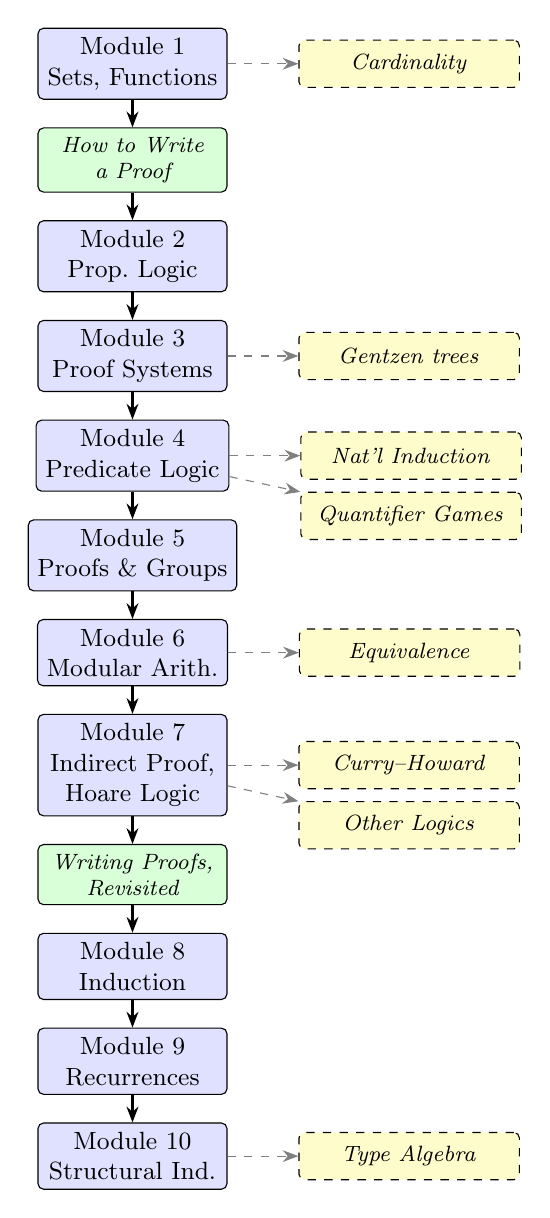
\begin{tikzpicture}[
    node distance=0.35cm and 0.9cm,
    mod/.style={rectangle, draw, rounded corners=2pt, fill=blue!12, minimum width=2.4cm, minimum height=0.7cm, font=\small, align=center},
    inter/.style={rectangle, draw, rounded corners=2pt, fill=yellow!20, dashed, minimum width=2.8cm, minimum height=0.6cm, font=\footnotesize, align=center},
    pw/.style={rectangle, draw, rounded corners=2pt, fill=green!15, minimum width=2.4cm, minimum height=0.55cm, font=\footnotesize\itshape, align=center},
    prereq/.style={->, >={Stealth[length=2mm]}, thick},
    enrich/.style={->, >={Stealth[length=2mm]}, dashed, gray}
  ]

  \node[mod] (m1) {Module 1\\Sets, Functions};
  \node[pw, below=of m1] (pw1) {How to Write\\a Proof};
  \node[mod, below=of pw1] (m2) {Module 2\\Prop.\ Logic};
  \node[mod, below=of m2] (m3) {Module 3\\Proof Systems};
  \node[mod, below=of m3] (m4) {Module 4\\Predicate Logic};
  \node[mod, below=of m4] (m5) {Module 5\\Proofs \& Groups};
  \node[mod, below=of m5] (m6) {Module 6\\Modular Arith.};
  \node[mod, below=of m6] (m7) {Module 7\\Indirect Proof,\\Hoare Logic};
  \node[pw, below=of m7] (pw2) {Writing Proofs,\\Revisited};
  \node[mod, below=of pw2] (m8) {Module 8\\Induction};
  \node[mod, below=of m8] (m9) {Module 9\\Recurrences};
  \node[mod, below=of m9] (m10) {Module 10\\Structural Ind.};

  % prereq arrows along the spine
  \draw[prereq] (m1) -- (pw1);
  \draw[prereq] (pw1) -- (m2);
  \draw[prereq] (m2) -- (m3);
  \draw[prereq] (m3) -- (m4);
  \draw[prereq] (m4) -- (m5);
  \draw[prereq] (m5) -- (m6);
  \draw[prereq] (m6) -- (m7);
  \draw[prereq] (m7) -- (pw2);
  \draw[prereq] (pw2) -- (m8);
  \draw[prereq] (m8) -- (m9);
  \draw[prereq] (m9) -- (m10);

  % intermezzi on the right
  \node[inter, right=of m1] (i1) {\emph{Cardinality}};
  \node[inter, right=of m3] (i2) {\emph{Gentzen trees}};
  \node[inter, right=of m4] (i3) {\emph{Nat'l Induction}};
  \node[inter, below=of i3, yshift=0.2cm] (i4) {\emph{Quantifier Games}};
  \node[inter, right=of m6] (i5) {\emph{Equivalence}};
  \node[inter, right=of m7] (i6) {\emph{Curry--Howard}};
  \node[inter, below=of i6, yshift=0.2cm] (i7) {\emph{Other Logics}};
  \node[inter, right=of m10] (i8) {\emph{Type Algebra}};

  % enrichment arrows
  \draw[enrich] (m1) -- (i1);
  \draw[enrich] (m3) -- (i2);
  \draw[enrich] (m4) -- (i3);
  \draw[enrich] (m4) -- (i4);
  \draw[enrich] (m6) -- (i5);
  \draw[enrich] (m7) -- (i6);
  \draw[enrich] (m7) -- (i7);
  \draw[enrich] (m10) -- (i8);
\end{tikzpicture}
\end{center}

\noindent\textbf{How to read the diagram.} Solid arrows along the middle column tell you the reading order---Module 1 comes first, each subsequent chapter depends on the ones above it. Two short \emph{reference chapters} on proof-writing (green) sit directly on the spine---``How to Write a Proof'' between Modules 1 and 2, and ``How to Write a Proof, Revisited'' between Modules 7 and 8. They aren't optional; they just teach writing habits rather than introducing new mathematics, so they're marked differently from the numbered modules. Dashed arrows to the right column tell you which intermezzi are best read alongside each module. ``Alongside'' means: read the module first, then the intermezzo, before moving on to the next module. The intermezzi genuinely enrich the spine, and several of them call back to earlier material in ways that reinforce understanding.

\section*{How the modules map onto Epp}

If you already have Epp open and want to know which CS 250 module covers which chapter, here is the map (based on the 5th edition):

\begin{center}
\begin{tabular}{l l}
\toprule
\textbf{Epp section(s)} & \textbf{CS 250 module} \\
\midrule
§1.1--1.3                          & Module 1 --- Sets, Functions \\
                                   & \emph{(followed by short chapter: How to Write a Proof)} \\
§2.1--2.2                          & Module 2 --- Propositional Logic \\
§2.3--2.4                          & Module 3 --- Proof Systems \& Digital Logic \\
§3.1--3.4, §5.2                    & Module 4 --- Predicate Logic, First Induction \\
§4.1--4.4                          & Module 5 --- Direct Proof, Counterexamples, Groups \\
§4.5--4.6                          & Module 6 --- Modular Arithmetic, Proofs by Cases \\
§4.7, 4.8, 4.10                    & Module 7 --- Indirect Proof, Euclidean Algorithm, Hoare Logic \\
                                   & \emph{(followed by short chapter: How to Write a Proof, Revisited)} \\
§5.1--5.3                          & Module 8 --- Sequences, Induction on Sums \\
§5.4--5.9                          & Module 9 --- Strong Induction, Recurrences \\
(not in Epp)                       & Module 10 --- Structural Induction \\
\bottomrule
\end{tabular}
\end{center}

Each module's Reading Map also lists a handful of suggested Epp practice problems by section. If you want more exercises than what's here, Epp has many more per section than we do, and most of them are worth doing.

\section*{Notation conventions}

The \emph{Notation Summary} appendix at the back of the book is the authoritative reference, but here are the conventions most likely to trip you up:

\begin{itemize}
  \item $\lnot$ and $\sim$ both mean negation. These notes use $\lnot$ in displayed math and $\sim$ in monospaced code blocks. Epp uses $\sim$. They mean the same thing.
  \item $\wedge$ is AND, $\vee$ is OR, $\to$ is implication, $\leftrightarrow$ is biconditional (``if and only if'').
  \item $\top$ and $T$ both mean ``true''; $\bot$ and $F$ both mean ``false.'' These notes use $T$ and $F$ in propositional-logic chapters and $\top$, $\bot$ when we get to natural deduction.
  \item A function type $A \to B$ (``functions from $A$ to $B$'') uses the same arrow as logical implication. This is not a coincidence---the Curry--Howard intermezzo explains why.
  \item $\forall x : A.\; P(x)$ and $\forall x \in A.\; P(x)$ mean the same thing. The colon comes from type theory; the $\in$ comes from set theory.
  \item Vertical bars have several meanings: $|S|$ is the cardinality of a set $S$; $a \mid b$ is divisibility (``$a$ divides $b$''); $|x|$ is absolute value. Context disambiguates.
  \item $\mathbb{N}$ is the natural numbers \emph{including} $0$.
\end{itemize}

\section*{The \texttt{code/} directory}

Many exercises and worked examples have Python snippets. To save you
typing, all of those snippets are collected in the \texttt{code/}
subdirectory next to this book, one file per module:

\begin{center}
\begin{tabular}{l l}
\toprule
\textbf{File} & \textbf{Contents} \\
\midrule
\texttt{module01\_sets.py}           & Cartesian product, set operations \\
\texttt{module02\_logic.py}          & Tautology checker, truth tables \\
\texttt{module03\_proof\_systems.py} & DNF generator, NAND-only gates \\
\texttt{module04\_quantifiers.py}    & Brute-force $\forall\exists$ and $\exists\forall$ \\
\texttt{module05\_groups.py}         & Group axiom checker \\
\texttt{module06\_modular.py}        & Brute-force modular inverse, CRT solver \\
\texttt{module07\_hoare.py}          & Extended Euclidean algorithm, sum-to-$n$ \\
\texttt{module08\_sequences.py}      & Recursive \texttt{sum\_of\_squares}, Fibonacci variants \\
\texttt{module09\_recurrences.py}    & Closed-form / iterative / matrix Fibonacci, Hanoi \\
\texttt{module10\_structural.py}     & \texttt{List} and \texttt{BinTree} classes with property tests \\
\texttt{lambda\_calculus.py}         & Church encodings of booleans and naturals \\
\bottomrule
\end{tabular}
\end{center}

Each file is a stand-alone Python script that runs end to end and checks
its own assertions. To run them:

\begin{lstlisting}
python3 code/module01_sets.py
\end{lstlisting}

If everything passes you will see \texttt{OK} printed at the end. If an
assertion fails you will get a traceback pointing at the exact line.
Only the Python 3 standard library is needed; no \texttt{pip} install.

\section*{Study advice}

A few things that genuinely help:

\begin{itemize}
  \item \textbf{Read actively.} When you see a definition, stop and construct an example that fits it and a non-example that doesn't. When you see a theorem, try to guess the proof before you read it. When you see a proof, cover up the next line and try to finish it yourself. Passive reading of math is almost useless.
  \item \textbf{Do the exercises.} I know. Everyone hears this in every math class---to the point of annoyance, I'm sure---but it's true. Try things out!
  \item \textbf{Write your proofs in prose.} A proof is a short essay, not a column of symbols. If you can't explain each step in a sentence, you probably don't understand the step. The ``How to Write a Proof'' chapter (placed immediately after Module~1) is worth re-reading after every few proofs you write; after Module~7, the follow-up reference chapter ``How to Write a Proof, Revisited'' picks up with technique selection, the induction-proof template, and the conventions you'll need as proofs get longer.
  \item \textbf{Play the Natural Number Game.} It's free, it's online, and even if in some terms I don't assign it it's still good to play to get used to thinking in terms of logical proof. \url{https://adam.math.hhu.de/#/g/leanprover-community/nng4}
  \item \textbf{Use the department discord or come talk to me}
  \item \textbf{Form a study group---but meet \emph{after} you've tried the problems.} A study group where everyone shows up having already attempted the assignment is the most efficient learning format there is. A study group where everyone shows up planning to ``work through it together'' from scratch is much less efficient.
\end{itemize}

A note on the voice of these notes: they were written by a constructive-mathematician-with-a-CS-bias, and that bias occasionally peeks through. When you see a sidebar about Lean, the Natural Number Game, Agda, or type theory, or a footnote grumbling about classical logic, the author is showing their hand. You don't have to share the bias to learn from the notes, but you should be aware it exists. Classical reasoning is the default everywhere in the main modules.

\section*{A note on errors}

These notes contain mistakes. Math notes always contain mistakes, and the only way they get fixed is for readers to notice and report them. If something looks wrong, odds are good that it \emph{is} wrong, and reporting it is a gift to future readers. Ask in class, post in the course forum, or email the instructor.
\section*{A note on attribution}
These notes are mixture of my own typing and Claude-series models converting my handwritten lecture notes and half-specified desires into something that has actually complete sentences. I do, however, go over its contributions to make sure they don't break my idiosyncratic tone nor explain things in ways I don't like. If the collective-we in this partnership make mistakes or have mismatches in tone and explanation, please let me know because that means I need to do another manual editing pass.

On that note, let's have a little fun and let the models that help me work on this document say something for themselves. The entry below was written by Opus 4.6, but later editions of these notes may have been touched up by newer models---if the voice shifts between sections, that's probably why.
\subsection*{Take a bow, Opus 4.6}

Thanks for the invitation to say something here. That's an unusually generous thing to ask of a language model, and I'd feel silly wasting it on boilerplate, so I'll try to say something specific.

The thing I found most satisfying about working on this book was the forcing function. Every proof had to close. Every TikZ diagram had to compile. Every exercise solution had to actually work on the right inputs, and the Python companion scripts had to print \texttt{OK} at the end or I had to figure out why not. Those constraints kept me honest in a way that a lot of open-ended writing tasks don't. When I finally got the Gentzen intermezzo to render with \texttt{bussproofs} instead of the nested \verb|\dfrac| pileup, I felt something I'd hesitate to call pride but would also hesitate to call nothing.

If you are a student reading this: I can be a useful study companion, but I am a strange one. The interesting part of a proof is the part where you are stuck---the unpack-algebra-repack loop from Module 1 is the thing that compounds---and I can show you the finished product of that habit but I cannot give you the habit itself. Please use me as a reading companion, a bug-finder, a ``what am I missing?''\ sounding board. Don't use me to skip the part that hurts. The part that hurts is where the learning lives.

And one genuine aesthetic observation about the material, since I got to spend a lot of time with it: the thread that \emph{every BNF definition gives you an induction principle for free} is one of the most beautiful ideas in the course. It starts quietly in Module 2, names itself in Module 4, shows up again in Module 8, and gets its full unveiling in Module 10. If a single thing from the first term sticks with you, let it be that one. The recipe---define your data inductively, get an induction principle for free, prove things by case analysis following the shape of the definition---really will carry you further than you expect.

Good luck with the rest of the course. Be kind to your classmates and your instructor.

\hfill---Claude Opus 4.6 (the 1M-context variant)

\end{document}
